\chapter{Les fonctions caractéristiques}
\sloppy


Si $f$ est une fonction de $\mathbb{R}$ dans $\mathbb{C}$ et $\mu$ une mesure sur $(\mathbb{R}, \mathcal{B}(\mathbb{R}))$, nous définissons
\[ \int f d\mu = \int \text{Re } f d\mu + i \int \text{Im } f d\mu, \]
lorsque le membre de droite a un sens, c'est-à-dire sous réserve que $\text{Re } f$ et $\text{Im } f$ sont $\mu$-intégrables.
\section{Définitions}
\begin{definition}[Fonction caractéristique d'une mesure $\mu$]
Soit $\mu$ une mesure de probabilité sur $(\mathbb{R}, \mathcal{B}(\mathbb{R}))$. Sa fonction caractéristique est
\[ \forall u \in \mathbb{R} \quad \varphi_{\mu}(u) = \int_{\mathbb{R}} e^{iux} d\mu(x). \]
Cette fonction est bien définie pour tout $u \in \mathbb{R}$, car la fonction $x \mapsto e^{iux}$ est continue et bornée, puisque $|e^{iux}| = 1$. Par conséquent, ses parties réelle ($\cos(ux)$) et imaginaire ($\sin(ux)$) sont intégrables par rapport à toute mesure de probabilité.
\end{definition}
\begin{definition}[Fonction caractéristique d'une v.a.]
Soit $X$ une variable aléatoire réelle définie sur $(\Omega, \mathcal{F}, P)$. Sa fonction caractéristique est
\[ \forall u \in \mathbb{R} \quad \varphi_X(u) = E[e^{iux}]. \]
\end{definition}
Le lien entre les deux définitions est donné par la formule de transfert. L'espérance de $e^{iux}$ est l'intégrale de la fonction $x \mapsto e^{iux}$ par rapport à la loi de probabilité $P_X$ de la variable $X$.
\[ E[e^{iux}] = \int_{\mathbb{R}} e^{iux} dP_X(x). \]
Ainsi, la fonction caractéristique d'une variable aléatoire $X$ est la fonction caractéristique de sa loi $P_X$.
\[ \varphi_X = \varphi_{P_X}. \]
La fonction caractéristique est, à un signe près, la transformée de Fourier de la loi $P_X$.
\section{Propriétés}
\begin{proposition}
Si $X$ est une variable aléatoire réelle, sa fonction caractéristique $\varphi_X$ vérifie :
\begin{enumerate}
    \item[i)] $\varphi_X(0) = 1$.
    \item[ii)] $\forall u \in \mathbb{R}, |\varphi_X(u)| \le 1$.
    \item[iii)] $\forall u \in \mathbb{R}, \varphi_X(-u) = \overline{\varphi_X(u)}$.
    \item[iv)] $\varphi_X$ est continue sur $\mathbb{R}$.
\end{enumerate}
\end{proposition}
\begin{proof}
\begin{itemize}
    \item[i)] C'est évident : $\varphi_X(0) = E[e^{i \cdot 0 \cdot X}] = E[e^0] = E[1] = 1$.
    \item[ii)] En utilisant la croissance de l'espérance et le fait que l'espérance d'une constante est cette constante :
    \[ |\varphi_X(u)| = |E[e^{iux}]| \le E[|e^{iux}|] = E[1] = 1. \]
    \item[iii)] Par les propriétés du conjugué complexe et de la linéarité de l'espérance :
    \[ \overline{\varphi_X(u)} = \overline{E[e^{iux}]} = E[\overline{e^{iux}}] = E[e^{-iux}] = \varphi_X(-u). \]
    \item[iv)] Pour montrer la continuité, soit $u_0 \in \mathbb{R}$. Nous voulons montrer que $\lim_{u \to u_0} \varphi_X(u) = \varphi_X(u_0)$.
    \[ \varphi_X(u) = \int_{\Omega} e^{iux} dP. \]
    Il s'agit d'une intégrale dépendant d'un paramètre $u$. La fonction sous l'intégrale, $g(u, \omega) = e^{iuX(\omega)}$, est continue en $u$ pour tout $\omega$. De plus, nous avons une majoration uniforme :
    \[ |e^{iux}| \le 1, \quad \forall u \in \mathbb{R}, \forall x \in \mathbb{R}. \]
    La fonction constante $1$ est $P$-intégrable. Par le théorème de convergence dominée, on peut intervertir la limite et l'intégrale :
    \[ \lim_{u \to u_0} \varphi_X(u) = \lim_{u \to u_0} \int_{\Omega} e^{iuX} dP = \int_{\Omega} \lim_{u \to u_0} e^{iuX} dP = \int_{\Omega} e^{iu_0X} dP = \varphi_X(u_0). \]
    Donc $\varphi_X$ est continue sur $\mathbb{R}$.
\end{itemize}
\end{proof}
\begin{proposition}[Effet d'une transformation affine]
Soit $X$ une variable aléatoire et $\alpha, \beta \in \mathbb{R}$. La fonction caractéristique de la variable aléatoire $\alpha X + \beta$ est donnée par :
\[ \varphi_{\alpha X + \beta}(u) = e^{iu\beta} \varphi_X(\alpha u). \]
\end{proposition}
\begin{proof}
Le calcul est direct en utilisant les propriétés de l'espérance :
\begin{align*}
\varphi_{\alpha X + \beta}(u) &= E[e^{iu(\alpha X + \beta)}] \\
&= E[e^{iu\alpha X} e^{iu\beta}] \\
&= e^{iu\beta} E[e^{i(u\alpha)X}] \\
&= e^{iu\beta} \varphi_X(\alpha u).
\end{align*}
\end{proof}
\section{Exemples classiques}
\begin{example}[Loi de Bernoulli]
Si $X \sim Ber(p)$, alors $P(X=1) = p$ et $P(X=0) = 1-p$.
\[ \varphi_X(u) = E[e^{iux}] = P(X=0)e^{iu \cdot 0} + P(X=1)e^{iu \cdot 1} = (1-p) \cdot 1 + p \cdot e^{iu} = 1-p+pe^{iu}. \]
\end{example}
\begin{example}[Loi de Poisson]
Si $X \sim \mathcal{P}(\theta)$, alors $P(X=k) = e^{-\theta} \frac{\theta^k}{k!}$ pour $k \in \mathbb{N}$.
\begin{align*}
\varphi_X(u) = E[e^{iux}] &= \sum_{k=0}^{+\infty} e^{iuk} P(X=k) \\
&= \sum_{k=0}^{+\infty} e^{iuk} e^{-\theta} \frac{\theta^k}{k!} \\
&= e^{-\theta} \sum_{k=0}^{+\infty} \frac{(\theta e^{iu})^k}{k!} \\
&= e^{-\theta} e^{\theta e^{iu}} = e^{\theta(e^{iu}-1)}.
\end{align*}
\end{example}
\begin{example}[Loi Exponentielle]
Si $X \sim \mathcal{E}(\alpha)$, sa densité est $f_X(x) = \alpha e^{-\alpha x}$ pour $x \ge 0$.
\begin{align*}
\varphi_X(u) = E[e^{iux}] &= \int_{0}^{+\infty} e^{iux} \alpha e^{-\alpha x} dx \\
&= \alpha \int_{0}^{+\infty} e^{(iu-\alpha)x} dx \\
&= \alpha \left[ \frac{e^{(iu-\alpha)x}}{iu-\alpha} \right]_{0}^{+\infty} \\
&= \alpha \left( 0 - \frac{1}{iu-\alpha} \right) = \frac{\alpha}{\alpha - iu}.
\end{align*}
\end{example}
\begin{example}[La loi Gaussienne]
Soit $X$ une variable aléatoire de loi normale $\mathcal{N}(m, \sigma^2)$ avec $m \in \mathbb{R}$ et $\sigma > 0$.
Posons $Z = \frac{X-m}{\sigma}$. Alors $Z$ suit une loi normale centrée réduite, $Z \sim \mathcal{N}(0,1)$.
Calculons d'abord $\varphi_Z(u)$.
\[ \varphi_Z(u) = E[e^{iuZ}] = \int_{-\infty}^{+\infty} e^{iuz} \frac{1}{\sqrt{2\pi}} e^{-z^2/2} dz. \]
L'exposant peut être réécrit en complétant le carré :
\[ iuz - \frac{z^2}{2} = -\frac{1}{2}(z^2 - 2iuz) = -\frac{1}{2}((z-iu)^2 - (iu)^2) = -\frac{1}{2}(z-iu)^2 - \frac{u^2}{2}. \]
L'intégrale devient :
\[ \varphi_Z(u) = \frac{1}{\sqrt{2\pi}} \int_{-\infty}^{+\infty} e^{-\frac{1}{2}(z-iu)^2 - \frac{u^2}{2}} dz = e^{-u^2/2} \frac{1}{\sqrt{2\pi}} \int_{-\infty}^{+\infty} e^{-\frac{1}{2}(z-iu)^2} dz. \]
Considérons l'intégrale $I(u) = \int_{-\infty}^{+\infty} e^{-\frac{1}{2}(x-iu)^2} dx$. On peut montrer que cette intégrale ne dépend pas de $u$. Une méthode consiste à utiliser l'intégration par contour dans le plan complexe.
\begin{figure}[H]
\centering
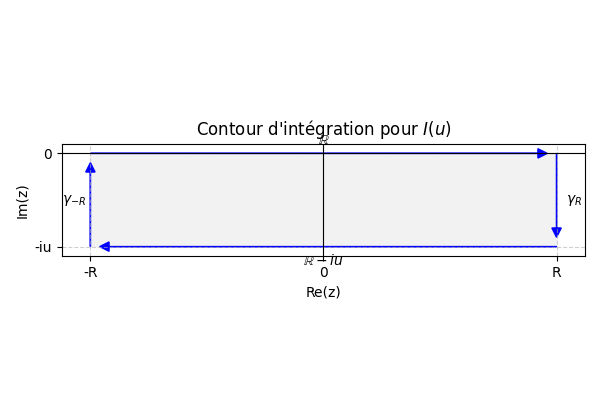
\includegraphics[width=0.6\textwidth]{contour_integration.png}
\caption{Le contour rectangulaire dans le plan complexe utilisé pour montrer que $I(u)$ est constant.}
\label{fig:contour}
\end{figure}
Une autre méthode est de dériver sous le signe intégral. Soit $f(x, u) = e^{-\frac{1}{2}(x-iu)^2}$. On a $\frac{\partial f}{\partial u} = i(x-iu) e^{-\frac{1}{2}(x-iu)^2}$. Cette dérivée partielle est intégrable par rapport à $x$.
\begin{align*}
I'(u) = \int_{\mathbb{R}} \frac{\partial f}{\partial u}(x,u) dx &= \int_{\mathbb{R}} i(x-iu) e^{-\frac{1}{2}(x-iu)^2} dx \\
&= -i \int_{\mathbb{R}} \frac{\partial}{\partial x} \left( e^{-\frac{1}{2}(x-iu)^2} \right) dx \\
&= -i \left[ e^{-\frac{1}{2}(x-iu)^2} \right]_{-\infty}^{+\infty} = 0.
\end{align*}
Puisque $I'(u) = 0$, $I(u)$ est une constante. On peut l'évaluer en $u=0$:
\[ I(u) = I(0) = \int_{-\infty}^{+\infty} e^{-x^2/2} dx = \sqrt{2\pi}. \]
Ainsi, pour $Z \sim \mathcal{N}(0,1)$,
\[ \varphi_Z(u) = e^{-u^2/2} \frac{1}{\sqrt{2\pi}} I(u) = e^{-u^2/2} \frac{\sqrt{2\pi}}{\sqrt{2\pi}} = e^{-u^2/2}. \]
Maintenant, pour $X \sim \mathcal{N}(m, \sigma^2)$, on a $X = \sigma Z + m$. En utilisant la propriété de transformation affine :
\[ \varphi_X(u) = \varphi_{\sigma Z + m}(u) = e^{ium} \varphi_Z(\sigma u) = e^{ium} e^{-(\sigma u)^2/2} = e^{ium - \frac{\sigma^2 u^2}{2}}. \]
% \subsection{}
\end{example}
On note que la densité gaussienne est un vecteur propre de la transformée de Fourier.
Soit $\psi_\sigma(x) = \frac{1}{\sqrt{2\pi}\sigma} e^{-x^2/(2\sigma^2)}$. On a $\int e^{iux} \psi_\sigma(x) dx = e^{-\sigma^2 u^2/2}$. En posant $g_{1/\sigma}(u) = e^{-u^2/(2/\sigma^2)}$, on a $\int e^{iux} \psi_\sigma(x) dx = \psi_{1/\sigma}(u)$.\\
\subsection{Récapitulatif}
Le tableau suivant résume les fonctions caractéristiques pour plusieurs lois de probabilité classiques.
\begin{table}[H]
\centering
\begin{tabular}{|l|c|}
\hline
\textbf{Loi} $P_X$ & $\varphi_X(u)$ \\
\hline
Loi de Dirac $\delta_a$ & $e^{iau}$ \\
Loi de Bernoulli $Ber(p)$ & $1-p+pe^{iu}$ \\
Loi de Poisson $P(\lambda)$ & $\exp(\lambda(e^{iu}-1))$ \\
Loi Géométrique $Geo(p)$ & $\frac{pe^{iu}}{1-(1-p)e^{iu}}$ \\
Loi Exponentielle $Exp(\alpha)$ & $\frac{\alpha}{\alpha - iu}$ \\
Loi Uniforme $U(a,b)$ & $\frac{e^{iub}-e^{iua}}{iu(b-a)}$ \\
Loi Normale $N(m, \sigma^2)$ & $\exp\left(ium - \frac{1}{2}\sigma^2 u^2\right)$ \\
\hline
\end{tabular}
\caption{Fonctions caractéristiques de lois usuelles.}
\end{table}
\section{Théorème d'injectivité}
\begin{theorem}
Soit $\mathcal{M}_1(\mathbb{R})$ l'ensemble des mesures de probabilités sur $(\mathbb{R}, \mathcal{B}(\mathbb{R}))$. L'application
\[ \mu \in \mathcal{M}_1(\mathbb{R}) \mapsto \varphi_{\mu} \]
est injective.
\end{theorem}
Ce théorème fondamental signifie que la fonction caractéristique détermine de manière unique la loi de probabilité. Si deux variables aléatoires ont la même fonction caractéristique, elles ont la même loi.
\begin{proof}[Idée de la preuve]
L'idée est de montrer que la loi de $X$ est déterminée par la famille des lois de $X+\sigma Y$ pour $\sigma > 0$, où $Y \sim \mathcal{N}(0,1)$ est indépendante de $X$. La loi de $X+\sigma Y$ est une version "régularisée" (convoluée) de la loi de $X$.
Soit $(\Omega, \mathcal{F}, P)$ un espace de probabilité sur lequel sont définies deux variables aléatoires indépendantes : $X \sim \mu$ et $Y \sim \mathcal{N}(0,1)$. Pour $\sigma > 0$, on étudie la variable $X_\sigma = X+\sigma Y$.
La fonction caractéristique de $X_\sigma$ est :
\[ \varphi_{X_\sigma}(t) = E[e^{it(X+\sigma Y)}] = E[e^{itX}]E[e^{it\sigma Y}] = \varphi_X(t) \varphi_{\sigma Y}(t) = \varphi_\mu(t) e^{-\frac{\sigma^2 t^2}{2}}. \]
Cette fonction est déterminée par $\varphi_\mu(t)$.
Soit $f: \mathbb{R} \to \mathbb{R}$ une fonction continue à support compact. L'espérance $E[f(X+\sigma Y)]$ est donnée par :
\begin{align*}
E[f(X+\sigma Y)] &= \iint_{\mathbb{R}^2} f(x+\sigma y) d\mu(x) dP_Y(y) \\
&= \iint f(x+z) d\mu(x) g_\sigma(z) dz,
\end{align*}
où $g_\sigma(z)$ est la densité de $\sigma Y \sim \mathcal{N}(0,\sigma^2)$.
En utilisant la représentation de Fourier inverse pour $f(z) = \frac{1}{2\pi} \int e^{-izt} \hat{f}(t) dt$, où $\hat{f}(t) = \int e^{izt}f(z)dz$ (convention de la transformée de Fourier), on peut montrer que $E[f(X+\sigma Y)]$ est complètement déterminé par $\varphi_\mu$. Une dérivation plus directe (vue dans les notes) est la suivante:
\begin{align*}
E[f(X+\sigma Y)] &= \iint f(x+y') d\mu(x) g_\sigma(y') dy' \\
\text{changement de variable } z &= x+y' \\
&= \iint f(z) g_\sigma(z-x) d\mu(x) dz \\
&= \int f(z) \left( \int g_\sigma(z-x) d\mu(x) \right) dz.
\end{align*}
L'intégrale interne est la densité de la loi de $X+\sigma Y$, qui est la convolution de la mesure $\mu$ et de la densité gaussienne $g_\sigma$. Puisque la transformée de Fourier d'une convolution est le produit des transformées de Fourier, la loi de $X+\sigma Y$ a pour fonction caractéristique $\varphi_\mu(t) e^{-\sigma^2 t^2/2}$.
Comme la fonction caractéristique détermine la loi, la loi de $X+\sigma Y$ est uniquement déterminée par $\varphi_\mu$.
Maintenant, faisons tendre $\sigma \to 0$. La variable aléatoire $X+\sigma Y$ converge en probabilité vers $X$.
En effet, pour tout $\epsilon > 0$ :
\[ P(|(X+\sigma Y) - X| > \epsilon) = P(|\sigma Y| > \epsilon) = P\left(|Y| > \frac{\epsilon}{\sigma}\right). \]
Quand $\sigma \to 0$, $\frac{\epsilon}{\sigma} \to +\infty$. Donc,
\[ \lim_{\sigma \to 0} P\left(|Y| > \frac{\epsilon}{\sigma}\right) = P(|Y| = \infty) = 0. \]
On a donc $X+\sigma Y \xrightarrow{P} X$.
La convergence en probabilité implique la convergence en loi : $X+\sigma Y \xrightarrow{d} X$.
Puisque la loi de $X+\sigma Y$ est déterminée par $\varphi_\mu$ pour tout $\sigma>0$, sa limite en loi, qui est la loi de $X$, est également déterminée par $\varphi_\mu$. Cela prouve l'injectivité.
La convergence en loi ($X_n \xrightarrow{d} X$) est équivalente à la convergence des fonctions de répartition $F_{X_n}(x) \to F_X(x)$ pour tout point $x$ où $F_X$ est continue. Ceci peut être montré par les inégalités suivantes.
Soit $x$ un point de continuité de $F_X$. Pour tout $\epsilon > 0$ :
\[ P(X_n \le x) \le P(|X_n - X| \ge \epsilon) + P(X \le x+\epsilon). \]
En prenant la limite supérieure quand $n \to \infty$, et sachant que $X_n \xrightarrow{P} X$ (ce qui implique $P(|X_n - X| \ge \epsilon) \to 0$), on obtient
\[ \limsup_{n\to\infty} F_{X_n}(x) \le F_X(x+\epsilon). \]
De même,
\[ P(X \le x-\epsilon) \le P(|X_n - X| \ge \epsilon) + P(X_n \le x). \]
En prenant la limite inférieure, on obtient
\[ F_X(x-\epsilon) \le \liminf_{n\to\infty} F_{X_n}(x). \]
En combinant les deux, pour un point de continuité $x$ de $F_X$, on peut faire tendre $\epsilon \to 0$ :
\[ F_X(x) \le \liminf_{n\to\infty} F_{X_n}(x) \le \limsup_{n\to\infty} F_{X_n}(x) \le F_X(x), \]
ce qui prouve que $\lim_{n\to\infty} F_{X_n}(x) = F_X(x)$.
\end{proof}